% This is a sample document using the University of Minnesota, Morris, Computer Science
% Senior Seminar modification of the ACM sig-alternate style. Much of this content is taken
% directly from the ACM sample document illustrating the use of the sig-alternate class. Certain
% parts that we never use have been removed to simplify the example, and a few additional
% components have been added.

% See https://github.com/UMM-CSci/Senior_seminar_templates for more info and to make
% suggestions and corrections.

\documentclass{sig-alternate}
\usepackage{xcolor}
\usepackage{hyperref}
\providecommand{\keywords}[1]{\textbf{\textit{Index terms---}} #1}

%%%%% Uncomment the following line and comment out the previous one
%%%%% to remove all comments
%%%%% NOTE: comments still occupy a line even if invisible;
%%%%% Don't write them as a separate paragraph
%\newcommand{\mycomment}[1]{}

\begin{document}

% --- Author Metadata here ---
%%% REMEMBER TO CHANGE THE SEMESTER AND YEAR
\conferenceinfo{UMM CSci Senior Seminar Conference, April 2014}{Morris, MN}

\title{Improving Security of Mobile Devices}

\numberofauthors{1}

\author{
% The command \alignauthor  (no curly braces needed) should
% precede each author name, affiliation/snail-mail address and
% e-mail address. Additionally, tag each line of
% affiliation/address with \affaddr, and tag the
% e-mail address with \email.
\alignauthor
Braden Luthi\\
	\affaddr{University of Minnesota, Morris}\\
	\affaddr{Morris, Minnesota, USA 56267}\\
	\email{luthi003@morris.umn.edu}
}

\maketitle
\begin{abstract}
	This paper gives an overview on three possible attack vectors (ways) to compromise the security of mobile devices and ultimately the privacy of the owner. These attacks include making use of weakness in older GSM systems to attack the newer UMTS systems, using mobile applications to secretly collect data such as key strokes, and using electromagnetic emissions from mobile devices to perform a ranged side-channel attack. For each of these attacks there will be a proposed solution to protect against the attacks, thereby increasing security of mobile devices.
	
\end{abstract}
\keywords{mobile security, Man-in-The-Middle, Application security, GSM, UMTS}

\section{Introduction}

As the number of mobile devices nears the number of people in the world, it should come as no surprise that mobile devices have become integral part of modern life. In fact nearly 25\% of average daily entertainment is spent using mobile devices, 80\% of consumers plan to conduct mobile commerce in the next 12 months, additionally PayPal mobile reported having handled over 14 billion dollars in 2012 alone. With this in mind it becomes ever more clear that mobile devices have become important not only our for entertainment purposes, but also for our financial purposes \cite{mobile-usage}. As processing power and usage continues to increase mobile devices have become evermore interconnected with our private information.  Not only do we allow our mobile devices to be so interconnected with our private data, but we load them with numerous third party applications (apps).   

%it is becoming ever more prevalent to be carrying around mobile devices boasting processors many times more powerful than the megalithic computers of the past. This processing power allows us to  access unimaginable amounts of information from thousands of hours of video, social media and news to personal financial information. 

With access to such volumes of private personal information with mobile devices it has become ever more prudent to insure the security of these devices. In this paper we will explore a number of security weaknesses that can potentially compromise the security of mobile devices and in turn the user's personal information beginning with a combination attack on the UMTS and GSM telecommunication standards, explained in Section \ref{GSM}. The attack makes use of weaknesses present in the older GSM system to attack the newer UMTS standard when the two systems interact. We conclude with a proposal for an additional procedure when dealing with interactions between the old and new systems. Continuing, we discuss security threats introduced with the wide-spread popularity of mobile applications and the threat that these applications may contain malicious software, such as a potential key-logging applications. We conclude with a software system that uses an apps permissions to warn against potentially malicious applications. Lastly we introduce an attack using relatively cheap radio equipment to gather electromagnetic (EM) emissions from the mobile device to perform a ranged side-channel attack.         

\section{Background}
	
Before explaining these attacks we introduce some background information on the GSM and UMTS telecommunication standards. In addition we briefly introduce the subject of cryptography and some of the attacks associated with it, mainly Man-in-the-middle and side-channel attacks.    	
	\subsection{GSM \& UMTS \label{GSM}}
	The Global System for Mobile Communications, or GSM, is a 2nd generation (2G) telecommunications standard developed by the European Telecommunications Institute in the early 90's. Since its deployment GSM has become one of the most widely used standards, reaching an 80\% market share at its height. GSM utilizes the A5 family of algorithms for data encryption, consisting of the A5/0 (no encryption), A5/1, A5/2 and A5/3 algorithms. A5/3 is considered to be the most secure followed by A5/1,A5/2 and A5/0 \cite{wiki:GSM}.  

The early 2000s saw the introduction of the Universal Telecommunications Standard or UMTS. UMTS is part of the third generation (3G) telecommunication standards developed by the 3rd Generation Partnership Project \cite{wiki:UMTS}. Based on GSM, UMTS employs a modified version of the A5/3 algorithm for encryption and has additional security features  that are not present in GSM. These features are discussed further in Section \ref{UMTS:Auth}. 

 As with any new technology such as 3G it takes a considerable amount of time to reach substantial levels of integration. A 2011 survey showed that nearly 90\% of the world's 1.2 billion mobile broadband subscribers were under 2G only coverage as compared to the 45\% coverage seen with 3G (3G/2G networks) technologies \cite{2G-coverage}. For 3G mobile devices to be able to travel long distances without losing coverage they need to be capable of interacting with the older 2G (GSM) networks and in fact most UMTS devices are capable of performing GSM. As GSM and other 2G infrastructure are replaced with 3G or even 4G equipment, service providers will need to continue to support older devices. This creates complex inter-operating networks which can introduce some unforeseen security issues as we will see in Section \ref{Handover}.

	\subsection{Cryptography \label{crypto}}
	Cryptography or  `secret writing' is the practice and study of techniques for securing communications between two parties by taking a message or \textit{plain-text} and turning it into something  unreadable known as \textit{cipher-text} by using some encryption algorithm and one or more keys. These keys are used to both encrypt and decrypt the message. It is commonplace to use what is known as a session key, which are keys that are used only for the duration of a conversation. Using session keys helps protect past and future conversations in the event that an attacker discovers a session key. In general modern-day cryptography is divided into two categories; symmetric cryptography, where both parties share a single secret key and asymmetric cryptography, where each individual has a secret private key and a public key. The public key is used for encrypting messages and the private is used for the decryption of messages.
	
	In cryptography there are several attacks which attempt to thwart encryption by either taking advantage of weaknesses inherent with the encryption algorithm or by taking advantage of the users. For example a cipher-text only attack refers to an attack that allows the attacker to discover the encryption key of a message using just the cipher-text. Since the whole idea of cryptography is to be able to send messages without fear of unwanted parties reading the message, cipher-text only attacks quite problematic. Other types of attacks include Man-in-the-middle attacks and side-channel attacks which will be discussed in more detail in the following subsections.   

\subsubsection{Man-in-the-middle Attack}	
In cryptography a Man-in-the-middle attack (MIM) is a type of an attack were an attacker tricks individuals into relaying messages between the participants and the attacker. The attacker accomplishes this by intercepting the initial key establishment messages, modifying the messages with the attacker's key  and then impersonating the participants to each other.. With this done all communication between the individuals will pass through the attacker enabling the attacker to not only listen in on the conversations but also manipulate and insert their own messages.

For example, consider two parties wanting to begin communication using  asymmetric cryptography. 
%
%
%
%
%
%

 As in Figure~\ref{MIM} let us call them Alice and Bob. In addition to Alice and Bob we also have an attacker Mallory, who wants to listen in on or even manipulate the conversation between Alice and Bob.
	\begin{description}
	\item[1.] Mallory intercepts Alice's message to Bob asking for his public key.\hfill\\\\
	$Alice$: ``Hi Bob, it's Alice send me your key" $\rightarrow$ $Mallory$
	\item[2.] Mallory relays the message to Bob; Bob cannot tell if the message is really from Alice \hfill\\\\
	 $Mallory$ ``Hi Bob, it's Alice send me your key" $\rightarrow$ $Bob$ 	
	\item[3.]Bob responds with his key \hfill\\\\
	$Mallory$ $\leftarrow$[key$_{bob}$]  $Bob$
	\item[4.] Mallory replaces Bob's key with her own, relays this to  Alice, claiming that it is Bobs key\hfill\\\\
	$Alice$ $\leftarrow$[key$_{Mallory}$] $Mallory$
	\item[5.]
	Believing communication is secure Alice sends Bob a message believing only he can read it. \hfill\\\\
	$Alice$ ``send \$2000 to account 2034"[key$_{Mallory}$] \\
	$~\quad\quad\quad\quad\rightarrow$ $Mallory$
	\item[6.] Because the message is encrypted with Mallory's key, Mallory can decrypt it, read and modify this message if she so desires, reencrypt it with Bob's key and Bob forward it to Bob who believes it is a secure message from Alice. \hfill\\\\
	$Mallory$ ``send \$2000 to account 1099"[key$_{Bob}$] $\rightarrow$ $Bob$
	\end{description}	
	\begin{figure}
		\centering
		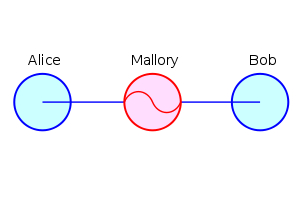
\includegraphics[scale=.5, bb= 65 65 250 250]{MIM.jpg}
		\caption[Man-In-The-Middle Attack]{Man-In-The-Middle Attack \cite{wiki:man}}
		 Communications from the participants (Alice and Bob) flows through the attacker (Mallory).
		\label{MIM}
		\end{figure}
		
\section{GSM/UMTS Handover Weakness }

	In this section I  will be describing a Man-in-the-middle attack (MIM) against GSM/UMTS systems described in Meyer \cite{Meyer:2004} which makes use of a cipher-text only attack on A5/2 \cite{Barkan}. With this an attacker can derive the session key to decrypt all communication using that key. To begin we will need a basic understanding of how the GSM and UMTS networks handle authentication and key agreement. In GSM/UMTS each mobile device has a secret key $K_{s}$ that is shared with the service provider or `home network'. $K_{s}$ is used for both authentication and to generate session keys for communication encryption.     
	\subsection{GSM Authentication \& Key Generation} 
		To authenticate a mobile device in GSM an authentication center (AC) in the service provider's network generates a challenge pair ($\mathit{RAND_{A},RES_{A}}$), as well as a 64-bit encryption key  $K_{ses}$.  $K_{ses}$ stays the same so long as no new authentication is performed, meaning the same key for encryption may be used for a long period of time. This itself is a bad idea because extended use of an encryption key can give an attacker the time and data needed to figure out the key. $\mathit{RAND_{A}}$ is a random number and $\mathit{RES_{A}}$ is a number generated from $\mathit{RAND_{A}}$ and $K_{s}$. The AC then transmits $\mathit{RAND_{A}}$ to the mobile device. The mobile device, like the AC, takes the $\mathit{RAND_{A} \text{ and } K_{s}}$ and generates $\mathit{RES_{M}}$ which it then sends back to the AC for confirmation. A mobile device is successfully authenticated if the $\mathit{RES_{A}}$ and the $\mathit{RES_{M}}$ are equivalent.
		
	 Once the mobile device is successfully authenticated by the AC, a security handshake occurs where the mobile device and the network decide upon the encryption algorithm they are going to use. The mobile device sends to the base station a list of the algorithms it supports. The base station then selects one of the algorithms to be used and relays that choice back to the mobile device. With these steps completed GSM communication can now begin.
		
	\subsection{UMTS Authentication \& Key Generation \label{UMTS:Auth}} 
		UMTS authentication and key generation work in a very similar manner as in GSM. However in UMTS there are a few differences. In UMTS there is an encryption key $C_{ses}$ and integrity key $I_{K}$ both of which are 128 bits in length. Unlike in GSM, UMTS has counters which are used to determine how many packets (portions of data) have been encrypted with the same $\mathit{C_{ses} \text{ or } I_{K}}$. Once one the counters reaches some operator-set limit, a new round of authentication is performed.
		
		 In addition to the encryption and integrity keys, there is an authentication token or $\mathit{A_{Token}}$ which is generated using $\mathit{SQN}$, a sequenced number shared between the mobile and network, and $k_{s}$. The token is used for network authentication to protect mobile devices against attackers trying to impersonate a network. The $A_{Token}$ is sent along with $\mathit{RAND_{A}}$ during authentication \cite{Meyer:2004}. The mobile device first performs network authentication by checking the last 64 bits of $\mathit{A_{Token}}$ known as the method authentication code ($\mathit{MAC}$). The mobile generates $\mathit{MAC}$ known as $\mathit{XMAC}$ using the $\mathit{SQN and C_{s}}$, $\mathit{MAC \text{is then checked against} XMAC}$. If they are equivalent the network is successfully authenticated $\mathit{SQN}$ is incremented and mobile authentication and key generation continues as in GSM \cite{security-mech}. While $\mathit{A_{Token}}$ helps protect UMTS only networks against Man-in the middle attacks it does not protect GSM/UMTS crossover networks. 
  
	\subsection{MIM attack on GSM}
	As noted in \cite{Meyer:2004} GSM is susceptible to a man-in-the-middle (MIM) attack. In which an attacker forces a mobile device to connect to a fake base station. This can  be done by broadcasting the mobile's home network's networking number or by drowning out the the signal of a legitimate base station forcing   a mobile to connect, because while in 'stand-by' mode  the mobile connects to the best received base station. With this done an attacker can effectively turn off all encryption by sending only A5/0 as a supported algorithm to the base station and the mobile device. This would allow an attacker to listen in on and modify any data traffic between the mobile device and the network.
	\subsection{GSM/UTMS Handover \label{Handover}}
	Although GSM is fairly old technology it is still used today as noted in Section \ref{GSM}. This means that the service providers network will have to handle both GSM and UMTS technologies to ensure greater coverage or roaming capabilities. This means that some coverage areas may have one or both GSM or UMTS base stations, as UMTS infrastructure continues to replace GSM. In order to ensure roaming capabilities of UMTS, a UMTS mobile device would need to be able to connect to either of these base stations. This also means that as GSM is replaced by UMTS, a GSM device would need to be able to connect to a UMTS base station. In order to accomplish this several procedures were developed to convert GSM keys into UMTS keys and vice versa. For example when a UMTS device connects with a GSM base station it needs to convert the encryption and integrity keys $\mathit{C_{ses}\text{ and } I_{K}}$ into the GSM encryption key $K_{ses}$.   
	
	In the following equations $\oplus$ is `exclusive or' and $\|$ is concatenation.
\begin{equation}
	\label{C_3}
	\mathit{K_{ses} = c_{3}(I_{K},C_{ses}) = C_{ses1} \oplus C_{ses2}\oplus I_{K1} \oplus I_{K2}}
\end{equation}

Here $C_{ses} \text{and} I_{K} $ are broken into  $C_{ses1},C_{ses2},I_{K1}\text{ and }I_{K2}$ each with a length of 64 bits; such that $C_{ses1}$ and $I_{K1}$ correspond to the first 64 bits of $C_{ses},I_{K}$ respectively and $C_{ses2},I_{K2}$ correspond to the last 64 bits.
 Similarly when a GSM device connects to a UMTS base station, the station would need to convert the the GSM keys into the UMTS $\mathit{C_{ses} \text{ and } I_{K}}$ keys. 
\begin{equation} 
\label{C_4}
	\mathit{C_{ses} = c_{4}(K_{ses}) = K_{ses} \| K_{ses}}
\end{equation}
\begin{equation}
\label{C_5}
	\mathit{I_{K} = c_{5}(K_{ses}) = K_{ses1}\oplus K_{ses2}\|K_{ses}\|K_{ses1}\oplus K_{ses2}}
\end{equation}

Here $K_{ses1} \text{ and } K_{ses2}$ are 32 bits and $K_{ses1}$ corresponds to the first 32 bits of $K_{ses1}$ and $K_{ses2}$ corresponds to the last 32 bits.
 
In addition to roaming UMTS supports what are known as session handovers, which allow uninterrupted use of a service while traveling, e.g., traveling whilst on talking to someone. There are several scenarios that can occur during hand over between UMTS and GSM. With handover between two UMTS base stations the current encryption and integrity keys $C_{ses},I_{K}$ are transmitted to the new base station and are then reused after hand over. Similarly when hand over between two GSM base stations occurs the $K_{ses}$ is reused after it is transmitted to the new base station. However, it should be noted that the encryption algorithm may not be the same as the one used before hand over. If the new base station does not support the encryption algorithm used before hand over then another security handshake occurs the results of which are indicated with a hand over command message. For example let us say the new base station only supports A5/0 and A5/1 algorithms. However the old base station supported and was using the A5/2 algorithm, then the algorithm would need to be changed before encryption could continue. 

 During handover of UMTS device between UMTS and GSM base station the UMTS keys would need to be converted using $c_{3}(C_{ses},I_{K})$ in equation \ref{C_3}. Similarly when a GSM device is handed over to a UMTS base station its encryption key would need to be converted to UMTS using $c_{4}(K_{ses}) \text{ and } c_{5}(K_{ses})$ from equations \ref{C_4} and \ref{C_5} respectively. Lastly it should be noted that encryption is disabled before handover, it will stay disabled as UMTS retains encryption used and every GSM base station is capable of A5/0 (no encryption).   
	
	This ability to cross over between UMTS and GSM networks leads to vulnerabilities in UMTS through GSM's vulnerability to a MIM attack. When handling crossover with either a UMTS or GSM device there are several cases described in \cite{Meyer:2004}, were an attacker can pose as a GSM base station. By using the cipher-text only attack on A5/2, described in \cite{Barkan}, recover the $K_{ses}$ which allows the attacker to break any previous and future communication encrypted with that $K_{ses}$.   
	\subsection{Solution}
	In order to thwart the vulnerabilities to UMTS that arise with handling of crossover between UMTS and GSM systems Meyer \cite{Meyer:2004} suggests introducing an additional authentication procedure to UMTS which would occur when a mobile device is being handed over between a UMTS base station and GSM base station. While the device is still connected to a UMTS base station, during handover, authentication and key generation would be performed. The keys would then be forwarded to the the new base station at the end of the handover procedure.
		
		
	%%% May not need to talk so indepth about these%%%	
%	\subsection{A5 algorithm family}
%		provide basic background on the A5 family of encryption algorithms used in GSM/UMTS This section will provide a simplified version of how the A5 algorithms work in general.
%	\subsection{Linear Feedback Shift Registar(LFSR)}
%		section will explain what an linear feedback shift register(LFSR) is and provide and example to explain how it works.
%		



\section{Application Threat to Security} 

 Mobile application development and retail has become an ever booming industry, as of 2013 developers have created nearly 800,000 apps in the App Store and more than a million apps on Google Play. In addition nearly 40 billion app downloads were reported from apple's App Store in the first quarter of 2013 alone \cite{Keylogging}. In addition to the sheer volume of apps available, people use an average of 6.5 apps are used daily and nearly 80\% of all mobile usage being used in apps, applications have clearly become an important part of a mobile devices \cite{mobile-usage}.  With all of this exposure to essentially unknown third-party apps we run the risk of introducing malicious software (malware) onto our devices, where it can gain access to our personal and financial information.

% add example of wallpaper app attack here 
 
  The rest of this section will introduce several different attacks,  beginning with a discussion on the a potential key-logging threat to Android devices via a third-party keyboard app by Mohsen et al. Key-logging refers to the collecting and subsequent storing or transmission of key strokes from a key board, which can then be used to view all typed information such as passwords. Ending this section will be a introduction of proposed software that can be used to help identify potentially malicious apps. 
  
  %It should be noted that most of the research presented is on devices using Google's Android operating system (OS). This may be attributed to Google's openness on app development, which in turn may attract more malicious software development.%  
	\subsection{Android Key-logging}
	\label{app}        
	The Android OS was first released in 2008. It was designed primarily with touch screens in mind. However early releases of the OS's keyboard had limited functionality. In subsequent updates more functionality was added to the key board, in addition to providing the necessary functions for third-party developers to begin creating their own keyboards. Essentially Android supported the development of third-party keyboards; spurring the development of customized keyboards with multi-language support, themed keyboards and keyboards designed for people with disabilities and health problems \cite{Keylogging}.
	
	Android utilizes a permission system, which forces apps to declare permissions to make API system calls. This provides access to system and to user data such as contacts, messages and even the camera. Required permissions are declared in the \textit{AndroidManifest.xml} file with a \textit{uses-permissions} tag. Permissions are granted by the user upon installation, once an installed an app's permissions can not be changed. For example the \textit{SEND\_SMS} tag allows an application to send text or SMS messages, which could potentially be used to send SMS messages to a premium number incurring charges on the mobile users account.
	
	 There are two types of permissions, regular permissions and dangerous permissions. Regular permissions are considered to be low-risk, presenting minimal risk to other apps, the system or the user and are granted automatically by the System. Dangerous permissions are those that grant access to private user data, such as contact lists or call history, or control over the device which could be harmful to the user as the aforementioned SMS messaging. Because of the harm these permissions can pose, the system displays these permissions upon installation where they are either accepted or denied by the user only \cite{Keylogging}.
	 
	  In the case of a key-logging keyboard app \cite{Keylogging} lists several types of storage methods and associated permissions a keyboard key-logging app would need.
	\begin{enumerate}
	\item Shared Preferences: Store private primitive data in key value pairs
	\item Internal Storage: store data on the device's data
	\item External Storage: store data on external storage
	\item SQLite Databases: Store structured data in a private database
	\item Network Connection: Store data on the web with a private network server
	\end{enumerate} 
	 
This would require at a minimum the permission have access to the internet and the ability to write to some sort of external storage, which allows for the sending of collected data to an attacker. It is not unreasonable to assume a mobile user, wishing to install a keyboard app, to grant these permissions to the app without really questioning the reasoning for these permissions. If the keyboard app contains any malicious code i.e. performs key-logging, all of the information, messages, user names, passwords and other private data would be recorded and transmitted to the developer, potentially giving them access to a range of different information such as email or bank accounts.

In order to detect and stop such potentially harmful key-logging keyboards described above Mohsen et al. \cite{Keylogging} describes a piece of software they called KBsChecker. KBsChecker is a tool that checks for any potential key-logging and notifies the user if it any are found. It does so by analyzing installed apps installation and permission information by using the Android \textit{PackageManager}, which contains information such as the app's name, package name, version and permissions. With this data it goes through and searches for any combination of permissions that would allow the app to perform a key-logging attack. Once it has found a potentially harmful combination of permissions it notifies the user by listing the app's name along with a description of the threat the app could posses.

 By taking this basic idea the KBsChecker presents it would not be to unrealistic to develop similar software that scans a mobile device's apps, before or after installation, for potentially harmful combinations of permissions for attacks other than key-logging. As with the KBsChecker notify the user, which would help to increase security of mobile devices against malicious apps.    
\section{Ranged Side-channel Attack}
\label{side}
Kenworthy et al. \cite{kenworthy} describes a study on possible side-channel attack against mobile devices. The attack utilizes the electromagnetic (EM) emissions from the devices emitted during cryptographic computation to reveal the secret keys.

\subsection{Side-channel Attack}
A side-channel attack is another type of attack in cryptography. Unlike a Man-in-the-middle attack that tricks users into revealing messages, a side-channel attack makes use of physical vulnerabilities of the machines preforming the encryption. There are several different types of side-channel attacks that make use of various kinds of physical data. For example there are timing attacks that measure the time computations take, power consumption attacks that monitor the varying power consumption of hardware, acoustic attacks which make use of sound generated during computation and electromagnetic attacks that read electromagnetic emissions during computation. The goal of all of these are to provide useful information about the encrypted communications by exploiting physical by-products of cryptographic processes. In many cases these attacks can reveal the secret key enabling one to decrytp all communications using the key  \cite{wiki:side-channel}.

For example Figure~\ref{Power} depicts a power analysis attack of the CPU during RSA computation. RSA is a widely used asymmetric cryptographic algorithm for establishment of keys between two parties for use with symmetric cryptographic encryption. RSA uses the square and multiply algorithm for faster and more efficient modular exponentiation of large numbers positive numbers.

\[\tag{Square and Multiply}
x^n = \left\{
  \begin{array}{lr}
    x(x^2)^{\frac{n-1}{2}} &  \text{: if n is odd} \\
    (x^2)^{\frac{n}{2}} & \text{: if n is even}
  \end{array}
\right.
\]

  As noted before, Figure~\ref{Power} depicts power analysis during RSA computation. The large spikes in power usage indicates time where computation is occurring. The short spike corresponds to a squaring and the longer spike corresponds to a square and multiply. These power spike can be used to reveal the secret key used during RSA, the short power spike corresponds to a 0 and the long power spike corresponds to a 1. The portion of the secret key depicted in Figure~\ref{Power} would therefore be 01. This process can be done throughout the whole operation of RSA to reveal the complete secret key \cite{springer}.


Generally side-channel attacks require physical access to the machine preforming the computation, making side-channel attacks rather difficult to preform. However in the rest of this section we will be exploring a side-channel attack that does not require direct physical access to the machine.    
 \begin{figure*}
		\centering
		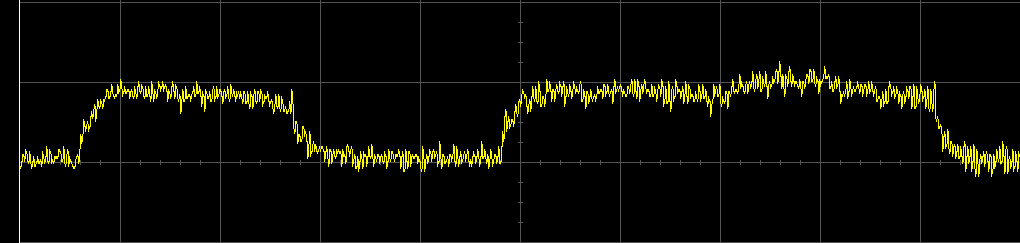
\includegraphics[scale=.5]{Power_attack.png}
		\caption{side-channel power analysis attack on RSA \cite{wiki:side-channel}}
		\label{Power}
		\end{figure*}
\subsection{The test}
In the study the authors analyzed several mobile devices from different manufacturers and OSs. Several different cyrptographic algorithms were implemented including RSA. During the study all other radio frequency (RF) channels were turned off by setting the devices in `airplane' mode, to ensure that any EM emissions leaking from the device are purely from unintended EM emissions from the CPU and not the the other RF transmissions.

To collect these EM emissions Kenworthy et al. used simple hardware and software costing around 1000 dollars. The hardware included magnetic field probe for close EM emissions, a Yagi antenna for far EM emissions, ICOM 7000 receiver, and an Ettus research USRP digitizer. In addition to this hardware the researchers developed simple custom software as well as some open source libraries for digital processing of the EM emissions.

 In all of the cases Kenworthy et al. were able to successfully discern the secret keys being used for all of the devices and algorithms. For example the keys from the devices using the RSA encryption were derived using a method similar to the power analysis as mentioned in the side-channel section. In particular the researchers were able to successfully perform this attack from a range of distances from a few cm away to over 10 feet way. The ranged properties of these attacks are particularly concerning as they over come the usual invasive qualities of side-channel attacks.
 
 To protect against such ranged attacks Kenworthy et al. suggest that implementations of cryptographic algorithms on mobile devices should incorporate known side-channel protection protocols, such as adding additional `dummy' operations in RSA during a squaring operation. This makes the squaring operation appear as a square and multiply operation and thus helps mask the actual operations and thus the secret key. In addition they mention the use of bulk encryption and authentication as `leakage tolerant cryptographic protocols'.      
\section{Conclusion}
As the popularity and usage of mobile devices continues to become more connected with the personal and financial information of users worldwide, security of these devices is only going to become an evermore important topic. The attacks described are just a handful of attacks that mobile devices today are vulnerable to. Security is not always easy to create ,as criminals are quite clever at finding and exploiting weaknesses. It is important that when developing security to keep in mind that there will inevitable be some way to exploit a weakness currently in mobile security. In addition we should strive to resolve these weaknesses as quickly as possible, for as mobile device usage and integration grows personal privacy becomes ever more reliant on security.     

\section{Acknowledgments}
\bibliography{Braden_Luthi_Sem_Paper} 
% The following two commands are all you need in the
% initial runs of your .tex file to
% produce the bibliography for the citations in your paper.
\bibliographystyle{abbrv}
% sample_paper.bib is the name of the BibTex file containing the
% bibliography entries. Note that you *don't* include the .bib ending here. 
% You must have a proper ".bib" file
%  and remember to run:
% latex bibtex latex latex
% to resolve all references

\end{document}
